% ============================================================
%  يُترجَم بـ XeLaTeX  (في Overleaf: Menu → Compiler → XeLaTeX)
%  الخط: Amiri (متوفر في Overleaf، أو حمّله من github.com/aliftype/amiri)
% ============================================================
\documentclass[12pt,a4paper]{article}
\usepackage[a4paper,margin=1.7cm,top=2.3cm,bottom=2.9cm,headheight=15pt,footskip=1.5cm]{geometry}
\usepackage{amsmath,amssymb}
\usepackage{icomma}
\usepackage[english,bidi=default,layout=lists]{babel}
\babelprovide[import,main]{arabic}
\babelfont{rm}[Scale=1.08]{Amiri}
\babelfont{sf}[Scale=1.08]{Amiri}
\usepackage[most]{tcolorbox}
\usepackage{tikz}
\usetikzlibrary{arrows.meta,calc,shadings}
\usepackage{array}
\usepackage{colortbl}
\usepackage{fancyhdr}
\usepackage{titlesec}
\usepackage{enumitem}
\usepackage{collcell}
\usepackage{needspace}
\usepackage{etoolbox}
% أعمدة جداول تُكتب خلاياها بالعربية في الاتجاه الصحيح
\newcolumntype{C}{>{\collectcell\ar}c<{\endcollectcell}}
% تجنب عنوان يتيم في أسفل الصفحة
\pretocmd{\section}{\Needspace{15\baselineskip}}{}{}
\pretocmd{\subsection}{\Needspace{11\baselineskip}}{}{}

% ---------- الألوان ----------
\definecolor{cDef}{HTML}{1F4E9C}
\definecolor{cThm}{HTML}{B3261E}
\definecolor{cRem}{HTML}{2E7D32}
\definecolor{cEx}{HTML}{C76B00}
\definecolor{cMeth}{HTML}{6A1B9A}
\definecolor{cSol}{HTML}{00695C}
\definecolor{cSec}{HTML}{1F3A68}

% ---------- العناوين ----------
\titleformat{\section}{\Large\bfseries\color{cSec}}{\thesection.}{0.6em}{}[{\color{cSec!60}\titlerule[1pt]}]
\titleformat{\subsection}{\large\bfseries\color{cThm!85!black}}{\thesubsection.}{0.5em}{}
\titlespacing*{\section}{0pt}{14pt}{8pt}
\titlespacing*{\subsection}{0pt}{10pt}{5pt}
\setlength{\parindent}{0pt}
\setlength{\parskip}{4pt}
\setlist{itemsep=2pt,topsep=3pt}

% ---------- الصناديق (تُرسم في سياق LTR ويُكتب محتواها بالعربية) ----------
\newtcolorbox{arbox}[3][]{enhanced,
  colback=#2!5,colframe=#2!80!black,arc=2mm,boxrule=0.8pt,
  left=6pt,right=6pt,top=8pt,bottom=5pt,
  fonttitle=\bfseries,coltitle=white,
  title={\foreignlanguage{arabic}{#3}},
  attach boxed title to top right={xshift=-5mm,yshift=-3mm},
  boxed title style={colback=#2!80!black,arc=1.5mm,boxrule=0pt},
  before upper={\selectlanguage{arabic}},
  before skip=8pt,after skip=8pt,breakable,#1}
\newenvironment{BOX}[2]{\begin{otherlanguage}{english}\begin{arbox}{#1}{#2}}{\end{arbox}\end{otherlanguage}}
\newenvironment{tarif}[1][تعريف]{\begin{BOX}{cDef}{#1}}{\end{BOX}}
\newenvironment{khassia}[1][خاصية]{\begin{BOX}{cThm}{#1}}{\end{BOX}}
\newenvironment{molahada}[1][ملاحظة]{\begin{BOX}{cRem}{#1}}{\end{BOX}}
\newenvironment{mithal}[1][مثال]{\begin{BOX}{cEx}{#1}}{\end{BOX}}
\newenvironment{tariqa}[1][طريقة]{\begin{BOX}{cMeth}{#1}}{\end{BOX}}

% ---------- التمارين والحلول ----------
\newcounter{exo}
\newenvironment{tamrin}[1]{\stepcounter{exo}\begin{BOX}{cSec}{التمرين \theexo: #1}}{\end{BOX}}
\newenvironment{hal}{\Needspace{12\baselineskip}\begin{otherlanguage}{english}\begin{arbox}[breakable]{cSol}{حل التمرين \theexo}}{\end{arbox}\end{otherlanguage}}

% رسومات TikZ تُوضع في سياق LTR
\newenvironment{LTR}{\begin{otherlanguage}{english}}{\end{otherlanguage}}
\newcommand{\ar}[1]{\foreignlanguage{arabic}{#1}}

% ---------- رموز ----------
% نقاط الحذف داخل الرياضيات (\dots يسبب خللاً في الاتجاه مع babel)
\renewcommand{\dots}{\mathinner{\ldotp\ldotp\ldotp}}
\renewcommand{\ldots}{\mathinner{\ldotp\ldotp\ldotp}}
\renewcommand{\cdots}{\mathinner{\cdotp\cdotp\cdotp}}
\newcommand{\N}{\mathbb{N}}
\newcommand{\Z}{\mathbb{Z}}
\newcommand{\D}{\mathbb{D}}
\newcommand{\Q}{\mathbb{Q}}
\newcommand{\R}{\mathbb{R}}
\newcommand{\pgcd}{\operatorname{PGCD}}
\newcommand{\ppcm}{\operatorname{PPCM}}

% ---------- تمثيل مجال على مستقيم عددي ----------
% \NLseg{a}{b}{[}{]}  مجال محدود
\newcommand{\NLseg}[4]{\begin{LTR}\begin{tikzpicture}[baseline=-0.6ex]
 \draw[-{Stealth[length=2mm]},gray!70](0,0)--(3.4,0);
 \draw[line width=2pt,cThm!80!black](0.7,0)--(2.7,0);
 \node[cThm!80!black,font=\LARGE] at (0.7,0){$#3$};
 \node[cThm!80!black,font=\LARGE] at (2.7,0){$#4$};
 \node[below=3pt,font=\footnotesize] at (0.7,0){$#1$};
 \node[below=3pt,font=\footnotesize] at (2.7,0){$#2$};
\end{tikzpicture}\end{LTR}}
% \NLright{a}{[}  مجال نحو +∞
\newcommand{\NLright}[2]{\begin{LTR}\begin{tikzpicture}[baseline=-0.6ex]
 \draw[-{Stealth[length=2mm]},gray!70](0,0)--(3.4,0);
 \draw[line width=2pt,cThm!80!black](1.3,0)--(3.3,0);
 \node[cThm!80!black,font=\LARGE] at (1.3,0){$#2$};
 \node[below=3pt,font=\footnotesize] at (1.3,0){$#1$};
\end{tikzpicture}\end{LTR}}
% \NLleft{b}{]}  مجال نحو −∞
\newcommand{\NLleft}[2]{\begin{LTR}\begin{tikzpicture}[baseline=-0.6ex]
 \draw[-{Stealth[length=2mm]},gray!70](0,0)--(3.4,0);
 \draw[line width=2pt,cThm!80!black](0.05,0)--(2.1,0);
 \node[cThm!80!black,font=\LARGE] at (2.1,0){$#2$};
 \node[below=3pt,font=\footnotesize] at (2.1,0){$#1$};
\end{tikzpicture}\end{LTR}}

% ---------- أيقونات مواقع التواصل (مرسومة بـ TikZ، لا تحتاج أي حزمة) ----------
\definecolor{cFB}{HTML}{1877F2}
\definecolor{cTG}{HTML}{229ED9}
\definecolor{cIG1}{HTML}{FEDA75}
\definecolor{cIG2}{HTML}{D62976}
\definecolor{cIG3}{HTML}{4F5BD5}
\newcommand{\fbicon}{\begin{LTR}\begin{tikzpicture}[baseline=-0.75ex,x=1em,y=1em]
 \fill[cFB] (0,0) circle (0.55);
 \node[white,inner sep=0,font=\usefont{TU}{lmss}{bx}{n}\small] at (0.04,-0.02) {f};
\end{tikzpicture}\end{LTR}}
\newcommand{\igicon}{\begin{LTR}
\begin{tikzpicture}[baseline=-0.75ex,x=1em,y=1em]
 \shade[lower left=cIG1,lower right=cIG2,upper left=cIG2,upper right=cIG3,rounded corners=0.28em] (-0.55,-0.55) rectangle (0.55,0.55);
 \draw[white,line width=0.09em,rounded corners=0.18em] (-0.36,-0.36) rectangle (0.36,0.36);
 \draw[white,line width=0.09em] (0,0) circle (0.17);
 \fill[white] (0.22,0.22) circle (0.05);
\end{tikzpicture}\end{LTR}}
\newcommand{\tgicon}{\begin{LTR}
\begin{tikzpicture}[baseline=-0.75ex,x=1em,y=1em]
 \fill[cTG] (0,0) circle (0.55);
 \fill[white] (-0.33,0.0) -- (0.32,0.27) -- (0.2,-0.3) -- (0.0,-0.15) -- (-0.08,-0.28) -- (-0.08,-0.08) -- cycle;
 \fill[cTG!70!black] (-0.08,-0.08) -- (0.25,0.2) -- (0.0,-0.15) -- (-0.08,-0.28) -- cycle;
\end{tikzpicture}\end{LTR}}
% سطر مواقع التواصل أسفل كل صفحة
% (يُكتب السطر بترتيب بصري من اليسار إلى اليمين: الأيقونة يمين كل اسم)
\newcommand{\PageBox}{\begin{LTR}\tikz[baseline=(p.base)]\node[fill=black,text=white,inner sep=2.5pt,minimum width=1.6em,minimum height=1.3em,font=\usefont{TU}{lmss}{bx}{n}\small](p){\ifnum\value{page}<10 0\fi\arabic{page}};\end{LTR}}
\newcommand{\SocialRow}{\begin{otherlanguage}{english}%
 \ar{\textbf{الأستاذ سوايسية هشام للرياضيات}}\ \tgicon\hfill
 \textbf{prof\_hicham\_math}\ \igicon\hfill
 \ar{\textbf{الأستاذ سوايسية هشام للرياضيات}}\ \fbicon\hspace{2.2em}\PageBox\end{otherlanguage}}
% ---------- رأس وتذييل الصفحة ----------
\pagestyle{fancy}
\fancyhf{}
\renewcommand{\headrulewidth}{0.6pt}
\renewcommand{\footrulewidth}{0.4pt}
% \SetHeader{يمين الرأس}{يسار الرأس}{يمين التذييل}{يسار التذييل}
\newcommand{\SetHeader}[2]{%
 \fancyhead[C]{\parbox{\textwidth}{\ar{#1\hfill #2}}}%
 \fancyfoot[C]{\parbox{\textwidth}{\small\SocialRow}}}

\usepackage{tkz-tab}
\usepackage{multicol}
% جدول تغيرات / إشارة (يُرسم في سياق LTR)
\newenvironment{TAB}{\par\begin{center}\begin{LTR}\begin{tikzpicture}[scale=0.95,every node/.style={font=\small}]}{\end{tikzpicture}\end{LTR}\end{center}}
% معلم بشبكة: \begin{GR}{xmin}{xmax}{ymin}{ymax}{unit cm}
\newenvironment{GR}[5]{\par\begin{center}\begin{LTR}\begin{tikzpicture}[x=#5cm,y=#5cm,font=\footnotesize]
 \def\xmn{#1}\def\xmx{#2}\def\ymn{#3}\def\ymx{#4}
 \draw[gray!25,very thin] (#1,#3) grid (#2,#4);
 \draw[-{Stealth[length=2mm]}] (#1,0)--(#2+0.3,0) node[below left]{$x$};
 \draw[-{Stealth[length=2mm]}] (0,#3)--(0,#4+0.3) node[below left]{$y$};
 \node[below left] at (0,0){$O$};
 \draw[very thick,-{Stealth[length=1.6mm]}] (0,0)--(1,0) node[below,pos=.55]{$\vec i$};
 \draw[very thick,-{Stealth[length=1.6mm]}] (0,0)--(0,1) node[left,pos=.55]{$\vec j$};
 \begin{scope}\clip (#1,#3) rectangle (#2,#4);}
{\end{scope}\end{tikzpicture}\end{LTR}\end{center}}
\newcommand{\Ticks}[2]{\foreach \t in {#1} \node[below,font=\scriptsize] at (\t,0){$\t$}; \foreach \t in {#2} \node[left,font=\scriptsize] at (0,\t){$\t$};}
\newcommand{\bx}[1]{\ensuremath{\colorbox{cDef!12}{$\displaystyle #1$}}}
\newcommand{\hl}[1]{\ensuremath{\colorbox{cEx!20}{$\displaystyle #1$}}}
\newcommand{\Lim}[1]{\displaystyle\lim_{x\to #1}}
\newcommand{\Cf}{(C_f)}
\newenvironment{qst}{\begin{enumerate}[label=\protect\circled{\arabic*},leftmargin=*]}{\end{enumerate}}
\newcommand{\circled}[1]{\foreignlanguage{english}{\tikz[baseline=(c.base)]\node[circle,fill=cDef,text=white,inner sep=1.2pt,font=\scriptsize\bfseries](c){#1};}}
% عمودان: \TwoCol{عرض اليسار}{محتوى اليسار}{عرض اليمين}{محتوى اليمين}  (آمن مع TikZ)
\newcommand{\TwoCol}[4]{\par\begin{LTR}\noindent\begin{minipage}[t]{#1\textwidth}\selectlanguage{arabic}#2\end{minipage}\hfill\begin{minipage}[t]{#3\textwidth}\selectlanguage{arabic}#4\end{minipage}\end{LTR}\par}
\newcommand{\un}{(u_n)}\newcommand{\vn}{(v_n)}
% برهان بالتراجع: \Rec{الخاصية P(n)}{التحقق من P(0)}{البرهان على الوراثة}
\newcommand{\Rec}[3]{\textbf{برهان بالتراجع:} نسمي $P(n)$ الخاصية: «#1».
\begin{itemize}
\item \textbf{التحقق:} #2
\item \textbf{الوراثة:} نفرض أن $P(n)$ صحيحة ونبرهن صحة $P(n+1)$: #3
\item \textbf{الخلاصة:} حسب مبدأ الاستدلال بالتراجع، $P(n)$ صحيحة من أجل كل عدد طبيعي $n$.
\end{itemize}}
\newcommand{\src}[1]{{\footnotesize\textbf{#1}}\par}
\newcommand{\ok}{$\textcolor{cRem}{\checkmark}$}
\newcommand{\limn}{\displaystyle\lim_{n\to+\infty}}
% أسئلة فرعية (أ) (ب) (جـ) كل سؤال في سطر
\newenvironment{sq}{\begin{itemize}[leftmargin=2.4em,itemsep=3pt]}{\end{itemize}}
\newcommand{\qa}{\item[(أ)]}\newcommand{\qb}{\item[(ب)]}\newcommand{\qc}{\item[(جـ)]}\newcommand{\qd}{\item[(د)]}\newcommand{\qe}{\item[(هـ)]}
\newcommand{\pa}{\par\smallskip\textbf{(أ)} }\newcommand{\pb}{\par\smallskip\textbf{(ب)} }\newcommand{\pc}{\par\smallskip\textbf{(جـ)} }\newcommand{\pd}{\par\smallskip\textbf{(د)} }\newcommand{\pe}{\par\smallskip\textbf{(هـ)} }
\newcommand{\ccl}[1]{\par\textbf{الخلاصة:} #1}

\pretocmd{\section}{\Needspace{24\baselineskip}}{}{}
\SetHeader{\small\bfseries\color{cSec}تمارين: الحساب الشعاعي ومعادلة مستقيم}{\small\color{cSec}السنة الأولى ثانوي -- جذع مشترك علوم وتكنولوجيا}
\begin{document}
\newcolumntype{M}[1]{>{\centering\arraybackslash}p{#1}}
\newcommand{\RL}[4]{\TwoCol{#3}{#4}{#1}{#2}}
\newcommand{\QQ}[1]{\par\smallskip\textbf{#1.} }
\newcommand{\ABC}[3]{\\[2pt]\begin{tabular}{p{0.28\textwidth}p{0.28\textwidth}p{0.28\textwidth}}(جـ) \ #3 & (ب) \ #2 & (أ) \ #1\end{tabular}}
\newcommand{\V}[1]{\overrightarrow{#1}}
\newcommand{\vu}{\vec u}\newcommand{\vv}{\vec v}
\newcommand{\cp}[2]{\begin{pmatrix}#1\\#2\end{pmatrix}}
\newcommand{\Ax}[4]{\draw[gray!25] (#1,#3) grid (#2,#4);
\draw[->] (#1-0.2,0)--(#2+0.3,0) node[right]{$x$}; \draw[->] (0,#3-0.2)--(0,#4+0.3) node[above]{$y$};
\foreach \t in {#1,...,#2} {\ifnum\t=0\else\node[below,font=\tiny] at (\t,0){$\t$};\fi}
\foreach \t in {#3,...,#4} {\ifnum\t=0\else\node[left,font=\tiny] at (0,\t){$\t$};\fi}
\node[below left,font=\tiny] at (0,0){$0$};}
\begin{LTR}
\begin{tcolorbox}[enhanced,colback=cSec,colframe=cSec,arc=3mm,halign=center,boxrule=0pt,top=12pt,bottom=12pt,before upper={\selectlanguage{arabic}}]
{\color{white}\fontsize{24}{30}\selectfont\bfseries سلسلة تمارين: الحساب الشعاعي ومعادلة مستقيم}\\[8pt]
{\color{white}\large تمارين متنوعة ونماذج فروض واختبارات -- بدون حلول (للتدرّب)}\\[5pt]
{\color{white}\large السنة الأولى ثانوي -- جذع مشترك علوم وتكنولوجيا}
\end{tcolorbox}
\end{LTR}

% =====================================================================
\section{الحساب الشعاعي دون معلم}
% ------------------------------------------------- 1
\begin{tamrin}{متوازي أضلاع ونقط معرّفة شعاعياً}
\begin{enumerate}
\item
\begin{sq}
\qa أنشئ متوازي الأضلاع $ABCD$ الذي مركزه $O$ حيث $AB=6\,cm$ و $AD=4\,cm$.
\qb أنشئ النقط $E$ ، $F$ و $G$ حيث: \ $\V{AE}=\dfrac14\V{AC}$ ، \ $\V{AF}=\dfrac13\V{DC}$ \ و \ $\V{OG}=\V{OC}-\V{OD}$.
\end{sq}
\item بيّن أن الرباعي $ABGO$ متوازي أضلاع.
\item
\begin{sq}
\qa بيّن أن: $\V{EB}+\V{ED}=2\V{EO}$ \ وأن \ $\V{EB}+\V{ED}=2\V{AE}$.
\qb استنتج أن النقطة $E$ هي منتصف $[AO]$.
\end{sq}
\item
\begin{sq}
\qa بيّن أن: $4\V{DE}=3\V{DF}$.
\qb هل النقط $D$ ، $E$ و $F$ في استقامية؟ علّل.
\end{sq}
\item
\begin{sq}
\qa برّر لماذا يمكن اعتبار $\big(A;\V{AO},\V{AB}\big)$ معلماً للمستوي.
\qb عيّن إحداثيات النقط $A$ ، $O$ ، $B$ ، $C$ ، $D$ ، $E$ ، $F$ و $G$ في هذا المعلم.
\qc باستعمال الإحداثيات تحقق من صحة النتائج 3(ب) و 4(ب).
\end{sq}
\end{enumerate}
\end{tamrin}

% ------------------------------------------------- 2
\begin{tamrin}{استقامية ومعلم كيفي}
$ABCD$ متوازي أضلاع ، نعتبر النقطتين $E$ و $F$ حيث: $\V{DE}=\dfrac52\V{DA}$ و $\V{CF}=\dfrac23\V{DC}$.
\begin{enumerate}
\item بيّن أن: $\V{BF}=\dfrac23\V{DC}+\V{BC}$ \ و \ $\V{BE}=\dfrac32\V{DA}-\V{AB}$.
\item اكتب الشعاعين $\V{BE}$ و $\V{BF}$ بدلالة الشعاعين $\V{AB}$ و $\V{BC}$.
\item بيّن أن $2\V{BE}+3\V{BF}=\vec0$. ماذا تستنتج؟
\item لتكن $A'$ نظيرة $A$ بالنسبة إلى $D$ ، و $M$ منتصف $[CD]$.
\begin{sq}
\qa بيّن لماذا يمكن اعتبار $\big(B;\V{BC},\V{BA}\big)$ معلماً للمستوي.
\qb عيّن إحداثيات النقط $A$ ، $B$ ، $C$ ، $D$ ، $M$ و $A'$ في هذا المعلم.
\qc بيّن أن النقطة $M$ هي منتصف القطعة $[BA']$.
\end{sq}
\end{enumerate}
\end{tamrin}

% ------------------------------------------------- 3
\begin{tamrin}{إنشاء نقط وعلاقات شعاعية}
$A$ ، $B$ و $C$ ثلاث نقط مختلفة مثنى مثنى وليست في استقامية.
\begin{enumerate}
\item علّم النقطة $D$ بحيث: $\V{DA}-3\V{DC}=\vec0$.
\item علّم النقطة $E$ بحيث: $\V{BE}=\V{BA}+\V{BD}$.
\item برهن أن $AEDB$ متوازي أضلاع.
\item برهن أنه من أجل كل نقطة $M$ من المستوي: \ $\V{MA}-3\V{MC}=-2\V{MD}$.
\item ليكن $O$ مركز متوازي الأضلاع $AEDB$. \ برهن أن: $\V{AB}+\V{AE}=2\V{AO}$.
\end{enumerate}
\end{tamrin}

% ------------------------------------------------- 4
\begin{tamrin}{منتصفات في متوازي أضلاع}
$ABCD$ متوازي أضلاع ، $E$ منتصف القطعة $[DC]$ و $F$ منتصف القطعة $[BC]$.
\begin{enumerate}
\item برهن أن: $\V{AC}+\V{BD}=2\V{BC}$.
\item عبّر عن $\V{AE}+\V{AF}$ بدلالة $\V{AC}$.
\end{enumerate}
\end{tamrin}

% ------------------------------------------------- 5
\begin{tamrin}{مثلث قائم وتعبير شعاعي}
$ABC$ مثلث قائم في $A$ حيث $AB=8\,cm$ و $AC=4\,cm$.
\begin{enumerate}
\item أنشئ النقطتين $L$ و $K$ حيث: $\V{AL}=\dfrac54\V{AB}$ و $\V{AK}=-\dfrac52\V{AC}$.
\item احسب $\big\|\V{AK}\big\|$ و $\big\|\V{AL}\big\|$ ، ثم استنتج $\big\|\V{KL}\big\|$.
\item $M$ نقطة من المستوي تحقق: $-\V{MA}+2\V{MB}+\V{MC}=\vec0$.
\begin{sq}
\qa عبّر عن $\V{AM}$ بدلالة $\V{AB}$ و $\V{AC}$ ، ثم أنشئ $M$.
\qb استنتج أن: $\V{AM}=\dfrac45\V{AL}-\dfrac15\V{AK}$.
\end{sq}
\end{enumerate}
\end{tamrin}

% =====================================================================
\section{الحساب الشعاعي في معلم}
% ------------------------------------------------- 6
\begin{tamrin}{مركبات ، ارتباط خطي ومعادلة مستقيم}
المستوي منسوب إلى معلم متعامد ومتجانس $(O;\vec i,\vec j)$. \ نعتبر النقط: $A(1;3)$ ، $B(-2;-3)$ ، $C(1;-1)$ و $D(3;\alpha)$ حيث $\alpha$ عدد حقيقي.
\begin{enumerate}
\item احسب مركبتي كل من الأشعة $\V{AB}$ ، $\V{BC}$ و $\V{AC}$ ، ثم أطوالها.
\item احسب مركبتي الشعاع $2\V{AB}+\V{BC}-\V{AC}$.
\item عيّن العدد الحقيقي $\alpha$ حتى يكون الشعاعان $\V{AB}$ و $\V{CD}$ مرتبطين خطياً.
\item اكتب معادلة للمستقيم $(AB)$ ، ثم معادلة للمستقيم $(\Delta)$ الذي يشمل $C$ ويوازي $(AB)$.
\end{enumerate}
\end{tamrin}

% ------------------------------------------------- 7
\begin{tamrin}{متوازي أضلاع ، استقامية وتوازي}
في معلم متعامد ومتجانس $(O;\vec i,\vec j)$ نعتبر النقط: $A(1;2)$ ، $B(-2;1)$ و $C(0;-2)$.
\begin{enumerate}
\item عيّن إحداثيي النقطة $D$ بحيث يكون الرباعي $ABCD$ متوازي أضلاع.
\item عيّن إحداثيي النقطة $M$ من المستوي بحيث: $\V{AM}=2\V{AB}-\V{AC}$.
\item نعتبر النقطة $N\Big(x;-\dfrac12\Big)$. \ عيّن قيمة $x$ حتى تكون النقط $C$ ، $B$ و $N$ في استقامية.
\item اكتب معادلة للمستقيم $(AB)$ ، ثم معادلة للمستقيم الذي يشمل $C$ ويوازي $(AB)$.
\end{enumerate}
\end{tamrin}

% ------------------------------------------------- 8
\begin{tamrin}{طبيعة مثلث ونقطة معرّفة شعاعياً}
في معلم متعامد ومتجانس $(O;\vec i,\vec j)$ نعتبر النقط $A$ ، $B$ و $C$ حيث: \ $\V{OB}=2\vec i+6\vec j$ ، \ $\V{OA}=-\vec i-\vec j$ \ و \ $\V{AC}\cp{6}{0}$.
\begin{enumerate}
\item عيّن إحداثيات النقط $A$ ، $B$ و $C$ ، ثم علّمها.
\item
\begin{sq}
\qa احسب الأطوال $AB$ ، $AC$ و $BC$.
\qb استنتج نوع المثلث $ABC$.
\end{sq}
\item احسب إحداثيي النقطة $N$ منتصف $[BC]$.
\item عيّن إحداثيي النقطة $M$ المعرّفة بالعلاقة: $\V{OM}=\V{AC}+2\V{NB}+\V{OC}$ ، ثم أنشئها.
\end{enumerate}
\end{tamrin}

% ------------------------------------------------- 9
\begin{tamrin}{مربع في معلم}
في معلم متعامد ومتجانس $(O;\vec i,\vec j)$ نعتبر النقط: $A(1;0)$ ، $B(3;-2)$ ، $C(3;2)$ و $E(5;0)$.
\begin{enumerate}
\item جد أطوال أضلاع المثلث $ABC$ ثم استنتج نوعه.
\item عيّن قيمة العدد الحقيقي $\alpha$ حتى تكون النقط $A$ ، $B$ و $D(\alpha;\alpha+1)$ في استقامية.
\item بيّن أن الرباعي $ABEC$ مربع.
\item
\begin{sq}
\qa جد معادلة المستقيم $(\Delta_1)$ الذي يشمل $B$ ويوازي $(AC)$.
\qb جد إحداثيي نقطتي تقاطع $(\Delta_1)$ مع محوري الإحداثيات.
\end{sq}
\item اكتب معادلة المستقيم $(\Delta_2)$ الذي يشمل $O$ ويوازي المستقيم ذا المعادلة $3x+2y+1=0$.
\item جد إحداثيي نقطة تقاطع $(\Delta_1)$ و $(\Delta_2)$.
\end{enumerate}
\end{tamrin}

% ------------------------------------------------- 10
\begin{tamrin}{متوازي أضلاع ، استقامية ومثلث قائم}
في معلم متعامد ومتجانس $(O;\vec i,\vec j)$ نعتبر النقط $A$ ، $B$ و $C$ حيث: \ $\V{OB}=-3\vec i-5\vec j$ ، \ $A(2;-2)$ \ و \ $\V{AC}\cp{-6}{2}$.
\begin{enumerate}
\item عيّن إحداثيي النقطة $C$ ، ثم علّم النقط $A$ ، $B$ و $C$.
\item عيّن إحداثيي النقطة $D$ حتى يكون الرباعي $ABCD$ متوازي أضلاع.
\item لتكن $M$ منتصف $[BC]$ ، والنقطة $N$ التي تحقق: $\V{DM}=\dfrac32\V{DN}$.
\begin{sq}
\qa استنتج أن النقط $D$ ، $M$ و $N$ في استقامية.
\qb عيّن إحداثيي النقطة $N$.
\end{sq}
\item اكتب معادلة للمستقيم $(\Delta)$ الذي يشمل $B$ ويوازي $(AC)$.
\item لتكن النقطة $E(-2;-4)$. احسب أطوال أضلاع المثلث $ACE$ ثم استنتج طبيعته.
\end{enumerate}
\end{tamrin}

% =====================================================================
\section{معادلة مستقيم ، وسيط وجمل معادلات}
% ------------------------------------------------- 11
\begin{tamrin}{مسألة شاملة: مستطيل ومستقيمات}
في معلم متعامد ومتجانس $(O;\vec i,\vec j)$ نعتبر النقط $A(-4;2)$ ، $B$ و $C$ حيث: $\V{OB}=-2\vec i+5\vec j$ و $\V{AC}\cp{8}{-1}$.
\begin{enumerate}
\item
\begin{sq}
\qa عيّن إحداثيي النقطة $B$ ، وبيّن أن $C(4;1)$ ، ثم علّم النقط $A$ ، $B$ و $C$.
\qb جد فاصلة النقطة $E$ التي ترتيبها $-1$ حتى تكون النقط $A$ ، $B$ و $E$ في استقامية.
\qc عيّن إحداثيي النقطة $F$ نظيرة $A$ بالنسبة إلى $B$.
\end{sq}
\item
\begin{sq}
\qa عيّن إحداثيي النقطة $D$ حتى يكون الرباعي $ABCD$ متوازي أضلاع.
\qb أثبت أن المثلث $ABC$ قائم في $B$ ، ثم استنتج بدقة طبيعة الرباعي $ABCD$ واحسب مساحته.
\end{sq}
\item
\begin{sq}
\qa اكتب معادلة ديكارتية للمستقيم $(AB)$ ، ثم استنتج معادلته المختصرة وعيّن معامل توجيهه.
\qb عيّن إحداثيي نقطتي تقاطع $(AB)$ مع محوري الإحداثيات.
\end{sq}
\item
\begin{sq}
\qa بيّن أن المعادلة $3x-2y=10$ هي معادلة للمستقيم $(T)$ الذي يوازي $(AB)$ ويشمل $D$.
\qb عيّن معادلة المستقيم $(d)$ الذي يشمل $D$ و $\V{AC}$ شعاع توجيه له.
\qc عيّن معادلة المستقيم $(\Delta)$ الذي معامل توجيهه $-\dfrac74$ ويشمل $C$ ، ثم تحقق أن $\V{FC}$ شعاع توجيه له.
\qd عيّن معادلة المستقيم $(T_1)$ الذي يشمل $B$ ويوازي محور الفواصل ، ومعادلة $(T_2)$ الذي يشمل $A$ ويوازي محور التراتيب.
\end{sq}
\item حل الجملة: $\begin{cases}3x-2y=-16\\x+8y=-14\end{cases}$ ، وفسّر النتيجة هندسياً.
\item $m$ عدد حقيقي ، و $(\Delta_m)$ المستقيم ذو المعادلة: $(m+3)x-(2m+1)y=-m$. \ عيّن $m$ في كل حالة:
\begin{sq}
\qa $(\Delta_m)$ يشمل النقطة $E$.
\qb $(\Delta_m)$ يوازي المستقيم $(T)$.
\qc $(\Delta_m)$ يوازي حامل محور التراتيب.
\qd معامل توجيه $(\Delta_m)$ هو $2$.
\end{sq}
\end{enumerate}
\end{tamrin}

% ------------------------------------------------- 12
\begin{tamrin}{متوازي أضلاع بوسيطين وعائلة مستقيمات}
المستوي منسوب إلى معلم متعامد ومتجانس. نعتبر $\alpha$ و $\beta$ عددين حقيقيين والنقط: $A(0;\beta^2)$ ، $B(\alpha-4;0)$ ، $C(-1;-\alpha^2)$ و $D(\beta;3)$.
\begin{enumerate}
\item جد قيمة كل من $\alpha$ و $\beta$ حتى يكون الرباعي $ABCD$ متوازي أضلاع.
\item نضع $\alpha=1$ و $\beta=2$ ، ولتكن النقطتان $E(-2;-6)$ و $W(-4;6)$.
\begin{sq}
\qa أثبت أن النقطة $E$ تنتمي إلى كل من المستقيمين $(BW)$ و $(AC)$.
\qb اكتب معادلة للمستقيم $(d)$ الذي يشمل $D$ ويوازي $(AC)$.
\end{sq}
\item $m$ وسيط حقيقي ، و $(\Delta_m)$ المستقيم ذو المعادلة: $y=\dfrac13(2m+1)x-m+2$.
\begin{sq}
\qa اكتب معادلة لكل من المستقيمين $(\Delta_0)$ و $(\Delta_{-1})$.
\qb أثبت أن جميع المستقيمات $(\Delta_m)$ تمر من نقطة ثابتة $L$ يطلب تعيين إحداثيها.
\qc عيّن $m$ حتى يشمل $(\Delta_m)$ النقطة $A$ ، ثم حتى يوازي $(\Delta_m)$ المستقيم $(d)$.
\end{sq}
\end{enumerate}
\end{tamrin}

% ------------------------------------------------- 13
\begin{tamrin}{عائلة مستقيمات تمر بنقطة ثابتة}
\RL{0.6}{%
لتكن $(\Delta_m)$ مجموعة النقط $M(x;y)$ من المستوي التي تحقق: $mx+(m-1)y+2=0$ ، حيث $m$ عدد حقيقي.
\begin{enumerate}
\item بيّن أنه من أجل كل عدد حقيقي $m$ فإن $(\Delta_m)$ مستقيم.
\item بيّن أن النقطة $A(-2;2)$ تنتمي إلى $(\Delta_m)$ من أجل كل $m$.
\item عيّن $m$ حتى تكون $B(1;1)$ من $(\Delta_m)$.
\item نفرض $m\ne1$. عيّن معامل توجيه $(\Delta_m)$.
\item عيّن $m$ حتى يكون $(\Delta_m)$ موازياً لـ $(d):10x+8y+5=0$.
\item ارسم $(\Delta_0)$ ، $(\Delta_1)$ و $(\Delta_2)$ في نفس المعلم.
\end{enumerate}}{0.37}{%
\begin{LTR}\centering
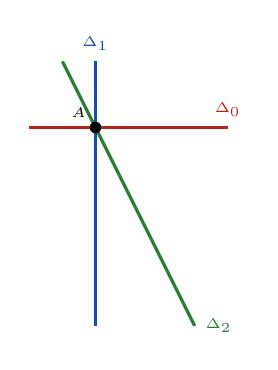
\begin{tikzpicture}[scale=0.42,font=\tiny]
\Ax{-4}{2}{-4}{4}
\draw[cThm,very thick] (-4,2)--(2,2) node[above]{$\Delta_0$};
\draw[cDef,very thick] (-2,-4)--(-2,4) node[above]{$\Delta_1$};
\draw[cRem,very thick] (-3,4)--(1,-4) node[right]{$\Delta_2$};
\fill (-2,2) circle (5pt) node[above left]{$A$};
\end{tikzpicture}
\end{LTR}}
\end{tamrin}

% ------------------------------------------------- 14
\begin{tamrin}{تعيين وسيط}
في معلم متعامد ومتجانس نعتبر النقط: $A(3;-4)$ ، $B(\alpha;5)$ و $C(3;0)$ حيث $\alpha$ عدد حقيقي.
\begin{enumerate}
\item عيّن قيمة $\alpha$ حتى تكون النقط $A$ ، $B$ و $C$ في استقامية.
\item عيّن إحداثيي النقطة $D$ حتى يكون الرباعي $AOCD$ متوازي أضلاع.
\item عيّن قيمة $\alpha$ حتى يكون معامل توجيه المستقيم $(BC)$ هو $2$.
\item عيّن قيمة $\alpha$ حتى يكون المستقيم $(BC)$ يوازي المستقيم الذي معادلته $y=-2x+5$.
\end{enumerate}
\end{tamrin}

% ------------------------------------------------- 15
\begin{tamrin}{جملة معادلتين وتقاطع مستقيمين}
\RL{0.6}{%
\begin{enumerate}
\item تحقق أن الجملة $(S):\begin{cases}x-y=-3\\-3x+y=-1\end{cases}$ تقبل حلاً وحيداً ، ثم حلها.
\item
\begin{sq}
\qa اكتب معادلة المستقيم $(D_1)$ الذي يشمل $A(-2;1)$ و $B(2;5)$.
\qb اكتب معادلة المستقيم $(D_2)$ الذي يشمل $C\Big(\dfrac13;0\Big)$ و $\vv\cp{1}{3}$ شعاع توجيه له.
\end{sq}
\item
\begin{sq}
\qa ارسم المستقيمين $(D_1)$ و $(D_2)$.
\qb من البيان عيّن نقطة تقاطعهما. ماذا تستنتج؟
\end{sq}
\end{enumerate}}{0.37}{%
\begin{LTR}\centering
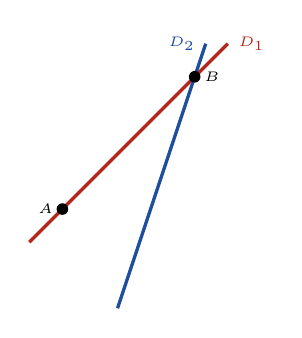
\begin{tikzpicture}[scale=0.42,font=\tiny]
\Ax{-3}{3}{-2}{6}
\draw[cThm,very thick] (-3,0)--(3,6) node[right]{$D_1$};
\draw[cDef,very thick] (-0.333,-2)--(2.333,6) node[left]{$D_2$};
\fill (2,5) circle (5pt) node[right]{$B$}; \fill (-2,1) circle (5pt) node[left]{$A$};
\end{tikzpicture}
\end{LTR}}
\end{tamrin}

% ------------------------------------------------- 16
\begin{tamrin}{وضعية: الطاولات والتلاميذ}
بمناسبة انتقاله إلى الثانوية نظّم يوسف وليمة دعا إليها تلاميذ قسمه. لاحظ أنه لو يجلس كل $5$ تلاميذ حول طاولة فإن $3$ منهم لا يجدون أماكن للجلوس ، ولو يجلس كل $6$ تلاميذ حول طاولة فإن $4$ طاولات تبقى شاغرة.\par
ما هو عدد التلاميذ الذين دعاهم يوسف؟ وما هو عدد الطاولات؟
\end{tamrin}

% =====================================================================
\section{اختيار من متعدد ، صحيح أم خطأ}
% ------------------------------------------------- 17
\begin{tamrin}{اختيار من متعدد}
اختر الإجابة الصحيحة الوحيدة مع التعليل (المعلم متعامد ومتجانس):
\begin{enumerate}
\item الشعاع $\V{AB}+\V{BC}+\V{CA}$ يساوي:
\ABC{$2\V{AC}$}{$\vec0$}{$\V{AB}$}
\item $A(1;2)$ و $B(3;-4)$. مركبتا $\V{AB}$ هما:
\ABC{$\cp{-2}{6}$}{$\cp{4}{-2}$}{$\cp{2}{-6}$}
\item منتصف $[AB]$ حيث $A(-1;4)$ و $B(3;0)$ هو:
\ABC{$(1;2)$}{$(2;2)$}{$(2;-2)$}
\item الشعاعان $\vu\cp{2}{-3}$ و $\vv\cp{-4}{k}$ مرتبطان خطياً من أجل:
\ABC{$k=-6$}{$k=6$}{$k=\dfrac32$}
\item معامل توجيه المستقيم المار بـ $(1;2)$ و $(3;8)$ هو:
\ABC{$3$}{$\dfrac13$}{$5$}
\item المستقيمان $y=2x+1$ و $4x-2y+5=0$:
\ABC{متوازيان}{متقاطعان}{متطابقان}
\item شعاع توجيه للمستقيم $3x-2y+1=0$ هو:
\ABC{$\cp{3}{-2}$}{$\cp{2}{3}$}{$\cp{-3}{2}$}
\item طول الشعاع $\vu\cp{3}{-4}$ هو:
\ABC{$7$}{$1$}{$5$}
\end{enumerate}
\end{tamrin}

% ------------------------------------------------- 18
\begin{tamrin}{صحيح أم خطأ}
أجب بصحيح أو خطأ مع التبرير:
\begin{enumerate}
\item إذا كان $\V{AB}=\V{DC}$ فإن $ABCD$ متوازي أضلاع (قد يكون مسطحاً).
\item إذا كانت $I$ منتصف $[AB]$ فإنه من أجل كل نقطة $M$: $\V{MA}+\V{MB}=2\V{MI}$.
\item النقط $A(1;1)$ ، $B(2;3)$ و $C(4;7)$ في استقامية.
\item المستقيم ذو المعادلة $x=3$ معامل توجيهه $0$.
\item النقطة $(2;-1)$ تنتمي إلى المستقيم $y=-2x+3$.
\item من أجل كل شعاعين $\vu$ و $\vv$: $\|\vu+\vv\|=\|\vu\|+\|\vv\|$.
\item إذا كان $\vu=-3\vv$ حيث $\vv\ne\vec0$ فإن $\vu$ و $\vv$ متعاكسان في الاتجاه.
\end{enumerate}
\end{tamrin}

\end{document}
